% =====================================================================
% PAPER 1, restyled to the register of the three IEEE WCL / COMML letters
% supplied by the author (Ajayan-Dash-Ramkumar, Dash-Mallik-Pandey, and the
% MIMO THz QKD paper).
%
% STYLE ONLY. Every claim, every number, every negative result and every
% % src: comment is carried over unchanged from
% paper/paper1/haatim_hsgs_letter.tex at 99a27e0. What changes is the voice:
%   - title in the "Performance Analysis of a ... System With ..." pattern;
%   - single-paragraph impersonal abstract ("is studied", "are derived");
%   - bold run-in headings replaced by lettered subsections and plain prose;
%   - a numbered contributions list introduced by the standard formula;
%   - a Numerical Results section that walks the figures in order;
%   - a Conclusion section carrying the limitations as prose.
%
% The frozen original is unchanged and remains the reference version.
% =====================================================================
\documentclass[journal]{IEEEtran}
\IEEEoverridecommandlockouts

\usepackage{amsmath,amssymb,amsfonts}
\usepackage{graphicx}
\usepackage{booktabs}
\usepackage{url}
\usepackage{xcolor}

% PROMPT 14 A3: \todo is NOT defined here. Nothing unresolved is allowed to
% render, and leaving the macro undefined makes a stray \todo a build error
% rather than red text that a tired author scrolls past. Open items live in
% docs/open-todos.md.

% Float placement: the default IEEEtran fractions leave a partly empty column
% wherever a float lands, which cost a page here. Relaxing them lets text share
% a page with a float. Layout only -- no content is affected.
\renewcommand{\topfraction}{0.92}
\renewcommand{\bottomfraction}{0.7}
\renewcommand{\textfraction}{0.06}
\renewcommand{\floatpagefraction}{0.85}
\renewcommand{\dbltopfraction}{0.92}
\renewcommand{\dblfloatpagefraction}{0.85}

\DeclareMathOperator{\rank}{rank}
\DeclareMathOperator{\range}{range}
\newcommand{\bG}{\mathbf{G}}
\newcommand{\bS}{\mathbf{S}}
\newcommand{\bB}{\mathbf{B}}
\newcommand{\bW}{\mathbf{W}}
\newcommand{\bZ}{\mathbf{Z}}
\newcommand{\bJ}{\mathbf{J}}
\newcommand{\bD}{\mathbf{D}}
\newcommand{\bU}{\mathbf{U}}
\newcommand{\bg}{\mathbf{g}}
\newcommand{\CN}{\mathcal{CN}}
\newcommand{\Hank}{\mathcal{H}}
\newcommand{\reff}{r_{\mathrm{eff}}}
\newcommand{\rmax}{r_{\max}}
\newcommand{\dhs}{\Delta_{\mathrm{HS}}}

\begin{document}

\title{Performance Analysis of a Hankel-Structured\\
Channel Estimator for Rydberg Atomic MIMO\\
Receivers With Magnitude-Only Observations}

\author{Abdullah~Haatim%
\thanks{A.~Haatim is with the Department of Electrical and Electronics
Engineering, Birla Institute of Technology and Science, Pilani~--- Pilani
Campus, India (e-mail: f20220519@pilani.bits-pilani.ac.in).}}

\maketitle

% Every number in this abstract is sourced where it is stated in the body:
% +2.93 / -0.25 / 0.163 dB -> Sec. IV-B; +2.46..+3.05 dB -> Sec. IV-A;
% 8.73 and ceil(N/2) -> Sec. I and Sec. II; 0.13 / 0.315 dB -> Sec. IV-E.
\begin{abstract}
Multi-user channel estimation for an atomic receiver measuring only the
magnitude of the incident field, in the presence of a known additive reference
beam, is studied in this letter. The problem is one of biased phase retrieval,
for which the Fisher information is shown to be rank one per measurement and
block diagonal across the receive elements, so that the normalised per-element
information is independent of the array size and the aperture is exploitable
only through cross-element structure. For a uniform linear array, the Hankel
lifting of each channel column supplies such a structure with a capacity of
$\lceil N/2\rceil$ ranks, from which it is predicted that a rank prior is
informative only when the channel occupies a small fraction of that capacity,
and harmful otherwise. An estimator enforcing this structure within an exact
expectation--maximization Gerchberg--Saxton iteration, with the model order
selected from a held-out pilot residual, is proposed. The predicted behaviour is
observed: a gain of $+2.93$~dB at $N=32$ and a loss of $0.25$~dB at $N=8$ in
summed squared error, averaged over twelve operating points per aperture, the
unstructured baseline varying by at most $0.163$~dB. The reversal is a property
of that statistic alone; under a paired per-trial median the same $N=8$ cells
yield $+0.225$~dB, the selector abstaining in $42\%$ of the trials.
The governing variable is shown to be the effective rank relative to capacity
rather than the path count, and predicts the gain on two channel distributions
to which it was not fitted, with errors of $0.13$ and $0.315$~dB. Results are
simulation only, and the derived bounds do not govern biased estimators.
\end{abstract}

\begin{IEEEkeywords}
Channel estimation, constrained Cram\'er--Rao bound, effective rank, Hankel
matrix, phase retrieval, Rydberg atomic receiver.
\end{IEEEkeywords}

\section{Introduction}

\IEEEPARstart{A}{tomic} receivers based on Rydberg states have emerged as a
promising technology for radio-frequency sensing and reception, since they read
out the incident field through an optical transition whose response is
proportional to the field \emph{magnitude}, thereby discarding the
phase~\cite{cui2025,gong2025mag}. Owing to this, multi-user channel estimation
in such receivers is a biased phase-retrieval problem, for which
Gerchberg--Saxton-type alternating projection~\cite{gerchberg1972} is the
natural solver. The atomic receiver enters only through the observation model
\eqref{eq:obs}, a magnitude-only measurement with a known additive reference;
nothing below depends on the vapour-cell physics, so the results apply to any
array receiver with that measurement.

Several studies on channel estimation for such receivers have been reported.
In~\cite{xiao2026}, the Gerchberg--Saxton iteration is unrolled into a trained
network. In~\cite{xu2025}, a rank projection is placed inside projected gradient
descent for the same problem, and the geometric channel model and path-count
distribution used here are specified. Structured low-rank Hankel recovery for
sums of exponentials has been studied outside this setting: EMaC
\cite{chen2014emac}, ALOHA \cite{jin2016aloha} and LORAKS
\cite{haldar2014loraks} recover such a matrix from \emph{partial linear}
observations by convex relaxation, while gridless line-spectrum and atomic-norm
methods~\cite{tang2013offgrid} likewise assume linear measurements and a
separation condition. Both families differ from the present setting in the same
way: the measurement here is a \emph{modulus}, so the map is not linear, no
convex relaxation applies, and the projection is a regulariser inside a
non-convex iteration rather than the estimator itself. No new projection
algorithm is claimed; Cadzow's composite property mapping~\cite{cadzow1988} is
used as given.

In this letter, we consider the conditions under which a structural prior is
informative for a magnitude-only estimator, organising the work around a single
argument stated first and tested afterwards. Under the unconstrained row-wise
parameterisation of \eqref{eq:obs} the Fisher information is block diagonal
across the receive elements, so the normalised per-element information does not
grow with $N$ and the aperture is usable only through cross-element structure.
On a uniform linear array (ULA) each path contributes one spatial complex
exponential, so the Hankel lifting of every channel column is rank
deficient~\cite{cadzow1988,markovsky2008} and admits at most
$\rmax(N)=\lceil N/2\rceil$ ranks, whence a rank prior is informative only when
the channel occupies a small fraction of that capacity. At $N=8$ the capacity is
$4$ while the path counts are $L_k\sim\mathcal{U}\{3,\dots,7\}$, so the constraint
is frequently vacuous and, when active, truncates genuine components. A sign
reversal at small $N$ is thus predicted rather than discovered afterwards, and
is reported as such in Section~\ref{sec:aperture} in summed squared error, the
quantity a bound governs; it does not appear in a median, for a reason made
precise in Section~\ref{sec:effrank}.

The remaining difficulty lies in determining when the channel does occupy a
small fraction of the capacity. An appeal to sparsity is unusable, since a
$16$-path channel on a $32$-element array is algebraically full rank yet has an
effective rank of
% src: reports/trackD_normalization.md:55, Track B Experiment C re-indexed;
% recomputed 8.694 at the same 200-trial budget, 8.669 at 1000 trials.
$8.73$, its lifting being compressible with nothing sparse about it. The path
count is accordingly replaced by the effective rank relative to capacity, which
is then tested prospectively. The major contributions of this letter can be
summarized as follows.
\begin{itemize}\setlength{\itemsep}{1pt}\setlength{\parskip}{0pt}
\item The Fisher information is derived and shown to be rank one per
measurement and block diagonal across the receive elements, and a
geometry-constrained bound is obtained in tangent-space form, the textbook form
being inapplicable owing to rank deficiency of the parameterisation.
\item The capacity $\rmax(N)=\lceil N/2\rceil$ is derived and the
aperture-scaling behaviour is presented as a test of a prediction made in
advance of the measurement.
\item The path-count heuristic is replaced by $\rho=\reff/\rmax$, with a
measurement separating the contribution of the \emph{prior} from that of the
\emph{estimator}.
\item Two cross-generator predictions registered before measurement are
reported, together with the pre-registered criteria that were not met.
\end{itemize}

\section{System Model and Proposed Estimator}
\label{sec:method}

Consider an $N$-element ULA serving $K$ single-antenna users over $P$ pilots.
With channel matrix $\bG\in\mathbb{C}^{N\times K}$, pilots $\bS$, known reference
beam $\bB$ and noise $\bW$, the received signal is given by
\begin{equation}
\bZ=\left|\bG\bS+\bB+\bW\right|,\qquad \bW_{np}\sim\CN(0,\sigma^2),
\label{eq:obs}
\end{equation}
where $|\cdot|$ denotes the elementwise magnitude operator. The modulus is
applied after the noise, owing to which \eqref{eq:obs} cannot be linearised. The
channel of each user is a sum of $L_k$ plane waves on the array manifold,
\begin{equation}
g_k[n]=\sum_{\ell=1}^{L_k}\alpha_{\ell,k}e^{-j(n-1)\psi_{\ell,k}},\qquad
\psi_{\ell,k}=\pi\sin\theta_{\ell,k},
\label{eq:chan}
\end{equation}
where $\jmath=\sqrt{-1}$, $L_k\sim\mathcal{U}\{3,7\}$~\cite{xu2025} and
$\theta\sim\mathcal{U}(-90^\circ,90^\circ)$. The reference-to-signal ratio (RSR)
is the reference power divided by the \emph{single-user} received power.

\subsection{Structure and Capacity of the Hankel Lifting}

Substituting \eqref{eq:chan} into the $(N-p)\times(p+1)$ Hankel lifting
$\Hank_p$ separates the exponential in the two indices, so each path contributes
one rank-one outer product and $\rank\Hank_p(\bg_k)\le L_k$. The maximum
admissible rank is therefore
\begin{equation}
\rmax(N)=\max_p\min(N-p,\,p+1)=\lceil N/2\rceil,
\label{eq:cap}
\end{equation}
and the constraint is vacuous whenever $L_k\ge\rmax(N)$. Note that $K$ cancels:
the structural model employs $3\sum_k L_k$ parameters against $2NK$, a ratio
independent of $K$, so the gain is expected to be $K$-invariant at fixed pilot
adequacy, as tested in Section~\ref{sec:kinv}.

\subsection{The Proposed Estimator}

The proposed Hankel-structured Gerchberg--Saxton (HS-GS) estimator applies,
after every exact expectation--maximization Gerchberg--Saxton (EM-GS) update, a
Cadzow projection $\mathcal{P}_r(\bg)=\Hank_p^{\dagger}(\Pi_r(\Hank_p(\bg)))$,
where $\Pi_r$ truncates to the $r$ leading singular values and
$\Hank_p^{\dagger}$ averages the antidiagonals. A single application is
\emph{not} idempotent, being one step of an alternating projection between the
rank set and the Hankel set, so the sweep count forms part of the definition of
the operator. The settings are not uniform across Section~\ref{sec:results}:
every result below is obtained at one of the four configurations of
Table~\ref{tab:config} and is tagged accordingly. All four employ
$n_{\mathrm{cz}}=4$ sweeps and differ in $T$ and the selection budget. With the
projection disabled, HS-GS reproduces EM-GS to $\max|\text{diff}|=0$, so the
projection is provably the only difference.

\subsection{Model Order Selection Without an Oracle}

A fraction $\nu=0.3$ of the pilot columns is held out, each candidate order
$r\in\{1,\dots,\rmax\}$ is scored by the held-out magnitude residual, and the
minimiser is retained. The in-sample residual cannot serve, since constraining
$\bG$ can only worsen the fit to the pilots used for fitting, so an in-sample
criterion always prefers the largest candidate. The true $L_k$ never enters, so
the rule uses no oracle. When the selector returns $\hat r\ge\rmax$ the
projection reduces to the identity and the estimator \emph{abstains}, falling
back exactly to EM-GS, a designed behaviour shown in Section~\ref{sec:effrank}
to be load-bearing.

Subspace methods such as root-MUSIC and ESPRIT recover $\{\psi_{\ell,k}\}$ from
% Named without a citation on purpose: see docs/open-todos.md item 2. The
% argument depends only on both methods needing the signal subspace, not on
% any specific result in those papers, and no verified entry exists here.
the signal subspace, but that subspace requires either multiple snapshots or the
complex field. With magnitude-only single-snapshot data it is identifiable only
\emph{after} phase retrieval has succeeded, at which point the channel is already
estimated. The exponential-sum manifold is therefore regularised toward rather
than parameterised.

Throughout, the primary statistic is the paired per-trial median within an SNR
bin, with bootstrap $95\%$ confidence intervals. Where a curve is compared
against a bound the ratio of summed errors is used, this being what a bound on
the mean-squared error governs; both are reported for the headline cell.

\begin{figure*}[!t]
\centering
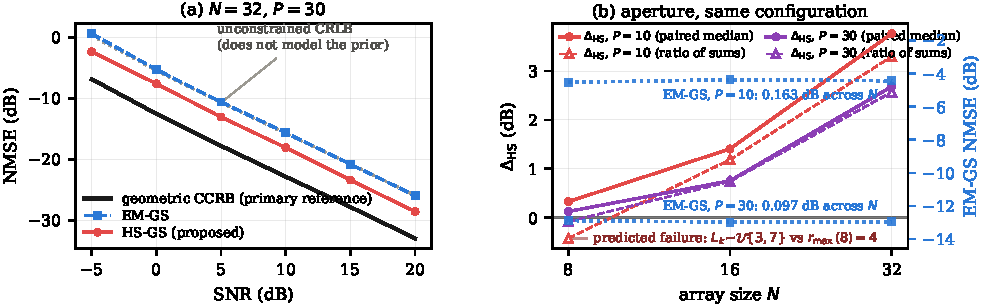
\includegraphics[width=\textwidth]{fig/fig1_twopanel_compact.pdf}
\caption{Configuration~A ($n_{\mathrm{cz}}=4$, $T=100$, budget $25$, RSR
$12$~dB, $K=3$, $400$ paired trials/point), both panels sharing one operator.
(a)~NMSE versus SNR at $N=32$, $P=30$; the unconstrained bound is faint since it
does not model the prior, and neither bound governs a biased estimator.
(b)~$\dhs$ versus $N$, each point the mean over six SNR values; filled markers
are the paired median, open markers the ratio of summed errors, the two
disagreeing at $N=8$.}
\label{fig:main}
\end{figure*}

\section{Performance Benchmark}
\label{sec:crlb}

\subsection{Rank-One Fisher Information}

Conditioned on $\bG$, $\bS$ and $\bB$ the noiseless field at $(n,p)$ is a
constant $\lambda$, so $z=|\lambda+w|$ is Rice distributed with a density
depending on $\lambda$ \emph{only through} $a=|\lambda|$. Denoting
$\frac{d}{dx}\log I_0(x)=R(x)$ and $\kappa=2za/\sigma^2$, the score is
$\partial_a\log p=\frac{2}{\sigma^2}[zR(\kappa)-a]$. Writing
$\beta=\sigma^{-4}(\mathbb{E}[z^2R^2(\kappa)]-a^2)$, one measurement carries the
scalar information $4\beta$, so in the real coordinates
$\boldsymbol\eta=[\Re\mathrm{vec}\,\bG;\Im\mathrm{vec}\,\bG]$,
\begin{equation}
\bJ_n=\sum_{p=1}^{P}4\beta(a_{n,p},\sigma^2)\,
\mathbf{u}_{n,p}\mathbf{u}_{n,p}^{T}.
\label{eq:fisher}
\end{equation}
Each magnitude measurement thus contributes rank-one and not rank-two
information. Crediting both quadratures overstates it and yields a bound too low
by
% src: results/track_b/constrained_crlb.json (unconstrained_rank1), 400 trials,
% the 36 points of the N x P x SNR grid shared by configurations A and B
$0.17$--$4.64$~dB across the $36$ operating points considered. An
identifiability check settles the form: at $K=3$, $P=3$ the per-row problem is
unidentifiable and \eqref{eq:fisher} is correctly singular, whereas the rank-two
construction claims full rank. Since the $n$-th row of $\bG\bS$ enters only the
$n$-th measurement row, $\bJ$ is \emph{block diagonal across the receive
elements}, so an unstructured estimator --- indeed any estimator attaining the
unconstrained bound --- is flat in $N$ under a normalised metric.

\subsection{Constrained Bound on the Geometric Manifold}

The unconstrained bound governs estimators treating $\bG$ as $2NK$ free
parameters. The proposed estimator instead exploits \eqref{eq:chan}, whose
parameters $\boldsymbol\phi\in\mathbb{R}^{3\sum_k L_k}$ number about $45$,
\emph{independent of $N$}. The textbook form $\bD(\bD^T\bJ\bD)^{-1}\bD^T$ with
$\bD=\partial\boldsymbol\eta/\partial\boldsymbol\phi$ is unusable, $\bD$ being
% src: results/track_b/constrained_crlb.json, mean jacobian_rank over the 12
% N=8 cells = 40.380; 3*mean(sum L_k) = 3 x 14.875 = 44.66; mean(3 sum L_k >
% 2NK = 48) over 6400 stored trials = 28.1%. Verified in
% reports/HSGS_PAPER_PROVENANCE.md:205-214.
rank deficient: at $N=8$ its mean numerical rank is $40.4$ against $\approx44.7$
parameters. The tangent-space form of~\cite{gorman1990,stoica1998} is therefore
employed, with $\bU$ an orthonormal basis of $\range(\bD)$,
\begin{equation}
\mathrm{CCRB}=\bU(\bU^T\bJ\bU)^{-1}\bU^T,
\label{eq:ccrb}
\end{equation}
which depends on the tangent \emph{space} and is invariant to
over-parameterisation. Both bounds are averaged over the same realisations as
the estimator curves.

Both bounds constrain the covariance of \emph{unbiased} estimators. All
estimators here run to a fixed budget with a shrinking update, and HS-GS also
truncates the rank, so none is unbiased and neither bound applies strictly. The
constrained bound is the primary reference in Fig.~\ref{fig:main}, being matched
to the estimator's model class; the unconstrained bound is secondary and governs
EM-GS only.

\section{Numerical Results}
\label{sec:results}

This section provides the numerical validation of the results derived above. For
the simulations, both estimators are handed identical realisations and $K=3$,
except where $K$ is the swept variable. Everything else varies by configuration,
so Table~\ref{tab:config} states the four in use and every number below carries
its label. Configurations A and B differ only in $T$ and the selection budget,
the one cell measured both ways differing by $0.005$~dB.
% src: reports/p12/PREREG_P22.md; results/p12/B1.json (T=100, ros mean 2.536)
% vs results/track_b/b3/N32_P30_snr*.npz (T=50, ros mean 2.531)

\begin{table}[!t]
\caption{Configurations used in Section~\ref{sec:results}: same estimator, same
held-out order rule ($\nu=0.3$, candidates $1..\rmax$, no oracle) and
$n_{\mathrm{cz}}=4$ sweeps throughout, differing only in operating point. TB $=$
Track~B, TD $=$ Track~D generator; ``$\mathcal{U}$'' denotes SNR drawn per trial
and binned post hoc. $^\dagger$$P$ is swept in the $K$-invariance ($13$--$27$)
and pilot-count ($10$--$35$) cells.}
\label{tab:config}
\centering
\scriptsize
\setlength{\tabcolsep}{2.5pt}
\begin{tabular}{lccccccll}
\toprule
 & $T$ & sel. & $P$ & RSR & Gen. & trials & SNR (dB) & used in \\
\midrule
A & 100 & 25 & 10, 30 & 12 & TB & 300--400 & $\{-5..20\}$ &
  \S\ref{sec:main}, \S\ref{sec:aperture}, \S\ref{sec:kinv} \\
B & 50 & 20 & 30 & 12 & TB & 400 & $\{-5..20\}$ &
  \S\ref{sec:kinv} (timing) \\
C & 100 & 25 & $20^\dagger$ & 10 & TD & 60--1000 & $\mathcal{U}[-10,20]$ &
  \S\ref{sec:effrank}--\S\ref{sec:kinv} \\
D & 50 & 20 & 30 & 12 & TB & 300 & $5$ &
  \S\ref{sec:pathcount}, \S\ref{sec:effrank} \\
\bottomrule
\end{tabular}
\end{table}

\subsection{Performance Against the Derived Bounds}
\label{sec:main}

In Fig.~\ref{fig:main}(a), the NMSE of both estimators is plotted against SNR
for configuration~A at $N=32$, $P=30$, together with the two bounds of
% src: results/p12/B1.json (bridging run), 400 trials/point, configuration A
Section~\ref{sec:crlb}. HS-GS improves upon EM-GS by $+2.46$ to $+3.05$~dB
across the sweep, with a six-point mean of $+2.68$~dB and a ratio-of-sums
improvement of $+2.33$ to $+2.96$~dB, the projection being active in $100\%$ of
the trials at this cell.

EM-GS tracks the
% src: results/track_b/constrained_crlb.json, N32_P30, vs results/p12/B1.json.
% The bounds depend on (N,P,K,RSR,SNR) and the generator, not on T or the
% selection budget, so they are common to configurations A and B.
unconstrained bound to within $0.143$~dB for SNR $\ge5$~dB, so it is informative
rather than vacuous. The constrained bound lies $7.05$--$7.11$~dB \emph{below}
it here, that gap being what the structural model is worth in principle; HS-GS
recovers part of it, remaining above the constrained bound at all six points by
$4.39$--$4.93$~dB.

\subsection{Aperture Scaling and the Choice of Statistic}
\label{sec:aperture}

Section~\ref{sec:crlb} predicts that the gain turns negative at small aperture.
In Fig.~\ref{fig:main}(b), $\dhs$ is plotted against $N\in\{8,16,32\}$ at
configuration~A, each point being the mean over $12$ operating points ($2$ pilot
counts $\times$ $6$ SNR values), so this panel and Fig.~\ref{fig:main}(a) share
one operator. The two pooling rules disagree at $N=8$ and agree elsewhere, so
both are
% src: results/p14/aperture_summary.json, configuration A, 400 trials/point;
% N=32 P=30 served from results/p12/B1.json (same cell, same operator)
reported below.

\begin{center}\footnotesize
\vspace{-2mm}
\begin{tabular}{cccc}
\toprule
$N$ & ratio of sums & paired median & EM-GS NMSE \\
\midrule
$8$  & $-0.254$ & $+0.225$ & $-8.705$ \\
$16$ & $+0.966$ & $+1.081$ & $-8.672$ \\
$32$ & $+2.934$ & $+3.226$ & $-8.700$ \\
\bottomrule
\end{tabular}
\vspace{-3mm}
\end{center}

\noindent It is evident that EM-GS varies by at most $0.163$~dB over the same
fourfold change in aperture, namely $0.163$~dB at $P=10$ and $0.097$~dB at
$P=30$, against a structured gain moving by over $3$~dB. Pooling the pilot
counts first yields $0.033$~dB, but the two move in opposite directions, so the
larger figure is quoted. This is what Section~\ref{sec:crlb} requires of an
estimator whose information is block diagonal in $N$.

The predicted reversal is a ratio-of-sums phenomenon. At $N=8$ the projection is
inactive in $41.8\%$ of the trials on average, rising from $12\%$ at $-5$~dB to
$59\%$ ($P=10$) and $79\%$ ($P=30$) at $+20$~dB as the selector declines a
constraint it cannot afford. Where active it truncates genuine components, and
the ratio of summed errors turns over accordingly, from $+1.272$~dB at $-5$~dB
to $-2.613$~dB at $+20$~dB for $P=10$, truncation bias not shrinking with the
noise while the variance term does. This is the predicted failure, measured.

The paired median does not reverse, and no claim is made that it does. At $N=8$
it is $+0.000$~dB at nine of the twelve points, positive and significant at the
other three, and negative and significant at none. The mechanism is that of
Section~\ref{sec:effrank}: abstention renders most trials bit-identical to EM-GS
and pins the median at zero, while the active minority dominates a sum of
squared errors. The prediction is therefore confirmed on the statistic a bound
governs and is \emph{invisible} to the one otherwise treated as primary. A
reader taking only the median away would conclude that the prior is never
harmful, and Section~\ref{sec:effrank} shows that it is not.

% src: reports/p12/p22_score.json
The bands registered before this sweep was run were $[-0.35,+0.05]$,
$[+0.60,+0.95]$ and $[+2.65,+3.00]$~dB. The values at $N=8$ and $N=32$ lie
inside their bands and that at $N=16$ misses by $0.016$~dB, so the
pre-registration failed. The EM-GS spread was predicted to be at most $0.15$~dB;
it is $0.033$~dB pooled, which the prediction named, and $0.163$~dB at $P=10$
alone, which would fail it. A failed prediction licenses no reporting other than
the measurement.

\subsection{Path Count as a Coordinate}
\label{sec:pathcount}

At configuration~D, holding $N=32$ and varying only the path count, with $L$
% src: trackB_hankel_emgs/results/experiment_C_path_count.csv, configuration D
identical across users at $5$~dB SNR, the gain decays monotonically from
$+7.04$~dB at $L=2$ to $-0.12$~dB at $L=16=\rmax$, while EM-GS moves by
$0.191$~dB in total. The operative variable is therefore channel complexity
relative to capacity, and aperture matters only because it sets that
capacity.

\subsection{Effective Rank, and the Prior Versus the Estimator}
\label{sec:effrank}

The path count is nevertheless imperfect, since clustered or unequal-strength
paths occupy fewer effective dimensions. The results are therefore indexed by
the Roy--Vetterli effective rank~\cite{royvetterli2007} of the lifting,
$\reff=\exp(-\sum_i p_i\ln p_i)$ with $p_i=\sigma_i/\sum_j\sigma_j$, normalised
as $\rho=\reff/\rmax$.

Re-indexing the sweep of Section~\ref{sec:pathcount} (configuration~D) moves
the zero crossing from $L/\rmax=0.90$ to $\rho=0.518$, and the useful region
becomes $\rho\lesssim0.5$, a statement about any channel rather than about the
$L$ values of one simulator. In Fig.~\ref{fig:boundary}, $\dhs$ is plotted
against $\rho$ for $N\in\{16,32,64\}$, the crossings being $0.588$, $0.518$ and
% src: reports/trackD_partB9_analysis.json B1_collapse; N=16,64 configuration C,
% N=32 configuration D. Crossings at N=16,64 are extrapolated, not bracketed.
$0.544$, a spread of $0.070$ over a fourfold change in aperture. This one
comparison spans two configurations, the $N=32$ value being at configuration~D
and the other two at configuration~C, and only the $N=32$ crossing is bracketed
on both sides, the other two being extrapolated from the positive side for the
reason given below.

The crossing belongs to the prior rather than to the estimator, and the two must
be stated separately. Past the crossing at configuration~C the paired per-trial
% src: results/p12/B2.json, 120-300 trials/cell, configuration C
median never becomes negative: at $\rho=0.608$ and $0.735$ for $N=16$ it is
$+0.078$ and $+0.000$~dB, and at
$\rho=0.596$ and $0.669$ for $N=64$ it is $+0.044$ and $+0.018$~dB. The reason
is abstention, since at $\rho=0.735$ the selector returns $\hat r\ge\rmax$ in
$38.8\%$ of the trials, the estimator then being exactly EM-GS. Forcing the
% src: results/p12/B2_forced.json -- DIAGNOSTIC ONLY, not the proposed method
projection active at that cell, as a diagnostic which is not the proposed
method, yields $-0.075$~dB, CI $[-0.186,-0.026]$. The prior therefore does
become harmful past the crossing, and abstention is what prevents the
\emph{typical} trial from following it down.

This does not contradict the negative values reported in
Sections~\ref{sec:aperture} and~\ref{sec:pathcount}; the difference is the
statistic, by the mechanism given there. Consequently, $\dhs\ge0$ is a property
of the selector under a median statistic only, and is neither evidence that the
prior is never harmful nor a guarantee concerning the mean-square error; where
the two disagree, both are reported.

The magnitude of the gain does not collapse onto the same axis. Over the window
% src: reports/trackD_partB9_analysis.json PRIMARY_internal_N16_vs_N64, config C
covered by both arrays at configuration~C, $N=16$ lies above $N=64$ by a mean of
$0.493$~dB and a maximum of $0.901$~dB, one-signed throughout, and no account of
this residual is offered. The one candidate tested, that the rank grid of the
% src: results/p12/B3.json, 250 trials/point, configuration C
selector is coarser at small capacity, is refuted: varying the pencil at fixed
$N=32$ and fixed $\rho$ gives a span of $0.390$~dB over admissible-rank counts
of $8$ to $16$ with \emph{no} monotone trend, the dependence running mildly
backwards. A pair with opposite matrix shapes but nearly equal rank counts,
$24\times9$ and $8\times25$, gives $+3.199$ and $+3.121$~dB, so the effect tracks
the rank count and not the shape.

Finally, $\rho$ is a design-time and not a receiver-observable coordinate, since
$\reff$ is computed on the noiseless channel. The abstention rate is observable
and monotone in $\rho$ at fixed aperture, but is confounded by capacity: at
% src: reports/p12/a3_abstention_vs_rho.json, 16 adaptive-order cells
$N=64$ a cell at $\rho=0.501$ abstains in $0.0\%$ of the trials while at $N=16$ a
% (both cells configuration C)
cell at $\rho=0.371$ abstains in $4.0\%$, so no single threshold separates the
useful region. An observable proxy therefore exists within an aperture but not
across apertures.

\begin{figure}[!htb]
\centering
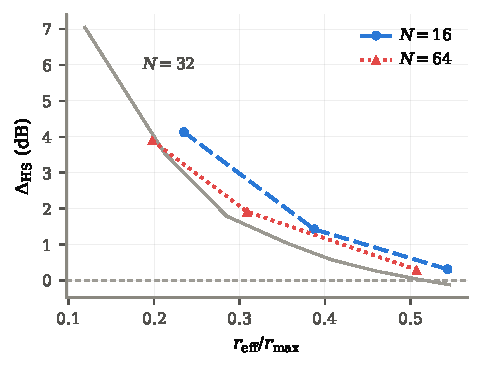
\includegraphics[width=0.86\columnwidth]{fig/fig2_boundary.pdf}
\caption{$\dhs$ versus $\rho=\reff/\rmax$ for $N\in\{16,32,64\}$. The boundary
location is stable across a fourfold change in aperture; the gain magnitude is
not, and that residual is unexplained.}
\label{fig:boundary}
\end{figure}

\subsection{Cross-Generator Prediction}
\label{sec:crossgen}

A relation fitted and evaluated on the same data proves little. The
$\rho$-to-gain relation was therefore frozen, numerical predictions were
committed to version control, and only then were two channel generators run
which had played no part in constructing it. The rule is a piecewise-linear
interpolation on a fixed eight-point table, with no regression and no spline, so
it re-executes exactly. Both tests employ the operator and operating point of
configuration~C with the generator replaced.

% src: reports/trackD_partB9_analysis.json, B6_xiao.B6_xiao_clustered
For a clustered Saleh--Valenzuela generator at $\rho=0.331$ the relation
predicted $+1.30$~dB, and the measurement over $276$ trials gave $+1.173$~dB, CI
$[+1.017,+1.380]$, an error of $0.13$~dB. For a second, independently specified
% src: reports/trackD_partB9_analysis.json, B8_cui_measured
configuration at $\rho=0.400$ the prediction was $+0.648$~dB with interval
$[+0.367,+1.015]$, and the measurement over $266$ trials gave $+0.963$~dB, CI
$[+0.808,+1.086]$, an error of $0.315$~dB, inside the stated interval but on its
upper edge.

These are \emph{cross-generator} and not out-of-model tests, since both
generators still produce channels of the form \eqref{eq:chan} and only the
distribution over $(L_k,\alpha_{\ell,k},\theta_{\ell,k})$ changes. They show that
$\rho$ transfers across path distributions, not that it survives a violation of
the ULA model.

\subsection{Users, Cost, and Placement of the Projection}
\label{sec:kinv}

% src: reports/trackD_partB9_analysis.json, cells B2_K{2,3,4}, configuration C
At configuration~C and fixed pilot adequacy $P/2K=3.33$, the gain varies by
$0.094$~dB across $K\in\{2,3,4\}$ for SNR $\ge5$~dB, corroborating the
$K$-invariance predicted in Section~\ref{sec:method}. Pooled over all SNR the
spread is $0.294$~dB against a pre-registered falsifier of $0.3$~dB, missed by
$0.006$~dB, and is reported rather than dropped.

% src: results/track_b/timing.json (config B); results/p12/B4.json (config C)
Order selection accounts for $57.7$--$85.5\%$ of the runtime. A coarse-to-fine
stride-$3$ search at configuration~C cuts that stage by $1.68\times$, from $16.0$
to $9.6$ candidate evaluations, and returns the same $\hat r$ in $93.3\%$ of the
trials, but missed its pre-registered criterion of at most $0.05$~dB, the
aggregate cost being $0.083$~dB. Its paired median degradation of $0.000$~dB
understates that cost, for the reason abstention does above, so it is reported
as an option which missed its gate and not as a validated substitute.

% src: results/p12/B5.json, 300 trials/point, shared \hat r, configuration A
Comparing interleaved projection against a single post-hoc Cadzow projection at
the same selected order, at configuration~A, interleaving is \emph{worse} at
$0$~dB ($-0.164$~dB, CI $[-0.317,-0.066]$), indistinguishable from $+5$ to
$+15$~dB, and better only at $+20$~dB ($+0.168$~dB, CI $[+0.102,+0.246]$), the
six-point mean being $+0.003$~dB. Interleaving is therefore not required in this
classical iteration, and no claim is made that it is.

Since placement is a wash, what the estimator contributes is not \emph{where}
the projection is applied but \emph{whether} it is applied at all and at what
order, decided from held-out pilots and using no oracle.
Section~\ref{sec:effrank} provides the evidence: the selector is what keeps
$\dhs\ge0$, and forcing the projection past the crossing costs $-0.075$~dB, CI
$[-0.186,-0.026]$. The order selector is thus the claim of this letter and not a
mechanism explained on the way to one.

\section{Conclusion}

Multi-user channel estimation for a magnitude-only atomic receiver with a known
additive reference is considered in this letter. The Fisher information is shown
to be rank one per measurement and block diagonal across the receive elements,
so the aperture is usable only through cross-element structure. The Hankel
lifting supplies such a structure with a capacity of $\lceil N/2\rceil$ ranks,
whence the prior helps only below a fraction of that capacity, and the predicted
sign reversal at small aperture is observed. The governing coordinate is
$\reff/\rmax$, whose boundary location is stable across a fourfold change in
aperture and which predicted the gain on two unseen channel distributions to
within $0.13$ and $0.315$~dB.

The scope is limited in the following respects. All results are obtained by
simulation only, with no measured hardware and no recorded channel data. They
cover geometric ULA channels of the form \eqref{eq:chan} at the array sizes,
pilot counts and generators tested, and the cross-generator tests change the
distribution but not the model family, so no claim is made beyond them. The
magnitude of the gain does not collapse onto the proposed axis, its residual of
$0.493$~dB being unexplained, and $\rho$ is not receiver-observable. Two of the
three boundary crossings cannot be bracketed from the negative side, since
abstention prevents it, and $\rho\approx0.75$ is unreachable at $N=64$, where the
% src: rydberg_sim/channel.py:245 raises above L=48 at N=64
path generator fails above $L=48$ ($\rho\approx0.67$). No fundamental bound is
established, since the derived bounds govern unbiased estimators while every
estimator here is biased.

% Three lines of the reference list would otherwise spill to a sixth page.
\enlargethispage{3\baselineskip}
\begin{thebibliography}{99}
\bibitem{cui2025} M.~Cui, Q.~Zeng, and K.~Huang, ``Towards atomic MIMO
receivers,'' \emph{IEEE J. Sel. Areas Commun.}, vol.~43, no.~3, pp.~659--673,
2025.

\bibitem{gong2025mag} T.~Gong \emph{et al.}, ``Rydberg atomic quantum receivers
for classical wireless communication and sensing,'' \emph{IEEE Wireless
Commun.}, vol.~32, no.~5, pp.~90--100, 2025.

\bibitem{gerchberg1972} R.~W.~Gerchberg and W.~O.~Saxton, ``A practical
algorithm for the determination of phase from image and diffraction plane
pictures,'' \emph{Optik}, vol.~35, pp.~237--246, 1972.

\bibitem{xiao2026} J.~Xiao, J.~Wang, M.~Zeng, H.~Xu, X.~Li, and
A.~Nallanathan, ``Channel estimation for Rydberg atomic quantum receivers:
unrolled phase retrieval from holographic snapshots,'' \emph{IEEE Signal
Process. Lett.}, vol.~33, pp.~1696--1700, 2026.

\bibitem{xu2025} B.~Xu, J.~Zhang, Z.~Chen, B.~Cheng, Z.~Liu, Y.-C.~Wu, and
B.~Ai, ``Channel estimation for Rydberg atomic receivers,'' \emph{IEEE Wireless
Commun. Lett.}, vol.~14, no.~9, pp.~2957--2961, 2025.

\bibitem{chen2014emac} Y.~Chen and Y.~Chi, ``Robust spectral compressed sensing
via structured matrix completion,'' \emph{IEEE Trans. Inf. Theory}, vol.~60,
no.~10, pp.~6576--6601, 2014.

\bibitem{jin2016aloha} K.~H.~Jin, D.~Lee, and J.~C.~Ye, ``A general framework
for compressed sensing and parallel MRI using annihilating filter based
low-rank Hankel matrix,'' \emph{IEEE Trans. Comput. Imag.}, vol.~2, no.~4,
pp.~480--495, 2016.

\bibitem{haldar2014loraks} J.~P.~Haldar, ``Low-rank modeling of local
$k$-space neighborhoods (LORAKS) for constrained MRI,'' \emph{IEEE Trans. Med.
Imag.}, vol.~33, no.~3, pp.~668--681, 2014.

\bibitem{tang2013offgrid} G.~Tang, B.~N.~Bhaskar, P.~Shah, and B.~Recht,
``Compressed sensing off the grid,'' \emph{IEEE Trans. Inf. Theory}, vol.~59,
no.~11, pp.~7465--7490, 2013.

\bibitem{cadzow1988} J.~A.~Cadzow, ``Signal enhancement---a composite property
mapping algorithm,'' \emph{IEEE Trans. Acoust., Speech, Signal Process.},
vol.~36, no.~1, pp.~49--62, 1988.

\bibitem{markovsky2008} I.~Markovsky, ``Structured low-rank approximation and
its applications,'' \emph{Automatica}, vol.~44, no.~4, pp.~891--909, 2008.

\bibitem{royvetterli2007} O.~Roy and M.~Vetterli, ``The effective rank: a
measure of effective dimensionality,'' in \emph{Proc. Eur. Signal Process.
Conf. (EUSIPCO)}, 2007, pp.~606--610.

\bibitem{gorman1990} J.~D.~Gorman and A.~O.~Hero, ``Lower bounds for parametric
estimation with constraints,'' \emph{IEEE Trans. Inf. Theory}, vol.~36, no.~6,
pp.~1285--1301, 1990.

\bibitem{stoica1998} P.~Stoica and B.~C.~Ng, ``On the Cram\'er--Rao bound under
parametric constraints,'' \emph{IEEE Signal Process. Lett.}, vol.~5, no.~7,
pp.~177--179, 1998.
\end{thebibliography}

\end{document}
